\documentclass{standalone}
\usepackage{tikz}
\begin{document}
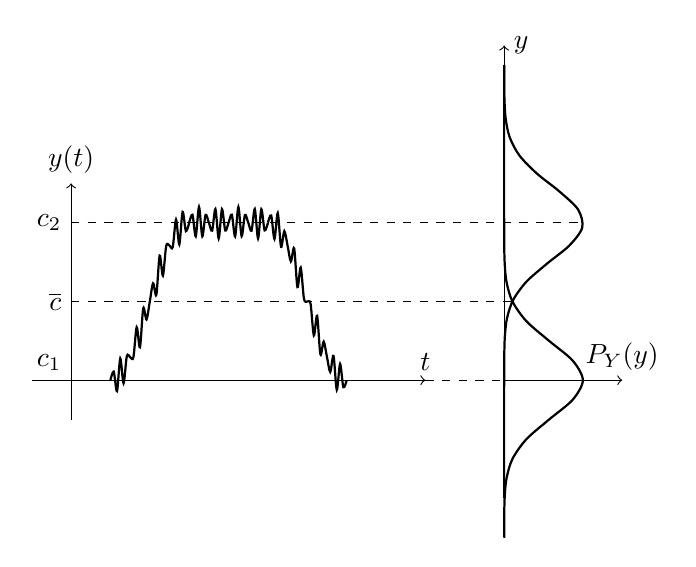
\begin{tikzpicture}[scale=2]
    \draw[thick,smooth, domain=-0.25:0.25]plot(\x,{1+0.1*sin(40*pi*(\x) r)});
    \draw[thick,smooth, domain=-0.75:-0.25]plot(\x,{1/2*(1+cos(2*pi*(abs(\x)-1/4) r))+0.1*sin(40*pi*(\x) r)});
    \draw[thick,smooth, domain=0.25:0.75]plot(\x,{1/2*(1+cos(2*pi*(abs(\x)-1/4) r))+0.1*sin(40*pi*(\x) r)});

    \draw[->](1.75,0)--(2.5,0)node[above]{$P_Y(y)$};
    \draw[->](1.75,-1)--(1.75,2.125)node[right]{$y$};
    \draw[dashed](-1,0.5)node[left]{$\overline{c}$}--(1.8,0.5);
    \draw[dashed](-1,1)node[left]{$c_2$}--(2.25,1);
    \draw[dashed](1.25,0)--(1.75,0);
    \node[above left]at(-1,0){$c_1$};
    \draw[->](-1.25,0)--(1.25,0)node[above]{$t$};    
    \draw[->](-1,-0.25)--(-1,1.25)node[above]{$y(t)$};

    \draw[thick,rotate=-90,smooth, domain=-2:0.75] plot (\x,{0.5*e^(-(3*(\x+1))^2)+1.75});
    \draw[thick,rotate=-90,smooth, domain=-2:1] plot (\x,{0.5*e^(-(3*\x)^2)+1.75});
\end{tikzpicture}
\end{document}